%
% 5-sobolevraum.tex
%
% (c) 2022 Prof Dr Andreas Müller, OST Ostschweizer Fachhochschule
%
\section{Sobolev-Räume
\label{buch:skalarprodukt:section:sobolev}}
\kopfrechts{Sobolev-Räume}
Im Beispiel~\ref{buch:skalarprodukt:hilbertraum:bsp:sinreihe} haben 
wir eine Reihe kennengelernt, deren Partialsummen alle stetig sind,
da sie trigonometrische Polynome sind.
Doch die Grenzfunktion ist die Rechteckfunktion, die ganz offensichtlich
nicht stetig sind.
Die Norm des Hilbertraums $L^2$ ist offenbar nicht stark genug, die
Stetigkeit der Grenzfunktion sicherzustellen.

\begin{figure}
\centering
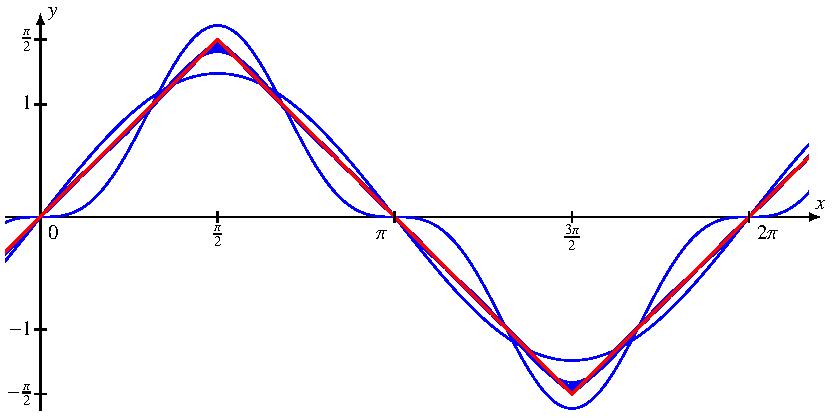
\includegraphics{chapters/010-skalarprodukt/images/fourierdreieck.pdf}
\caption{Die 
Reihe~\ref{buch:skalarprodukt:sobolevraum:eqn:fourierdreieck}
mit beliebig oft stetig differenzierbaren Partialsummen konvergiert
gleichmässig gegen die stetige Dreiecksfunktion, aber die Grenzfunktion
ist nicht mehr überall differenzierbar.
\label{buch:skalarprodukt:sobolevraum:fig:fourierdreieck}}
\end{figure}
Die Supremum-Norm ist zwar stärker, gleichmässig konvergente Folgen
von stetigen Funktionen konvergieren gegen einen stetigen Grenzwert.
Aber sie ist nicht stark genug Differenzierbarkeit zu erzwingen.
Die Reihe
\begin{equation}
f(x)
=
\frac{4}{\pi}\biggl(
\sin x - \frac{\sin 3x}{3^2} + \frac{\sin 5x}{5^2} -\frac{\sin 7x}{7^2} +\dots
\biggr)
\label{buch:skalarprodukt:sobolevraum:eqn:fourierdreieck}
\end{equation}
hat beliebig oft stetig differenzierbare Partialsummen und sie konvergiert
gleichmässig gegen die stetige, aber an den Stellen $k\frac{\pi}2$,
$k\in\mathbb{Z}$, nicht differenzier Dreicksfunktion (siehe
Abbildung~\ref{buch:skalarprodukt:sobolevraum:fig:fourierdreieck}).

Die Beispiele zeigen, dass Stetigkeits- und Differenzierbarkeitseigenschaften
beim Arbeiten in einem Hilbertraum verloren gehen könnten.
Andererseits möchte man einen Hilbertraum dazu verwenden,
Differentialgleichungen zu lösen, wo man aus der Theorie weiss, dass
die Lösungen beliebig oft stetig differenzierbar sind.
Es ist daher anzunehmen, dass wir diese als Grenzfunktionen bezüglich
einer stärkeren Norm erhalten können, welche die Differenzierbarkeit
garantiert.
In diesem Abschnitt sollen die wesentlichen Ideen der Konstruktion
dieser sogenannten Sobolev-Räume skizziert werden.

%
% Ableitungen
%
\subsection{Ableitungen}

%
% Skalaraprodukt mit Ableitungen
%
\subsection{Skalarprodukt mit Ableitungen}

%
% Konvergenz der Ableitungen
%
\subsection{Konvergenz der Ableitungen}





